% Original incident simulation, with invented times and server names.
\documentclass[10pt,aspectratio=169]{beamer}
\usetheme{Singapore}
\usecolortheme{whale}
\usepackage{amsmath,tikz,listings}
\usetikzlibrary{arrows.meta,positioning}
\setbeamertemplate{navigation symbols}{}
\setbeamercolor{alerted text}{fg=orange!80!black}
\lstset{basicstyle=\ttfamily\small,columns=fullflexible,keepspaces=true}
\title{Why a timeout is not a verdict}
\subtitle{A distributed-systems incident review}
\author{Systems reliability workshop}
\date{Incident simulation 10}
\begin{document}
\begin{frame}[plain]\titlepage\end{frame}
\section{Reconstruct}
\begin{frame}{At 10:02, the client did not receive an answer}
\begin{columns}[T]
\begin{column}{.47\textwidth}\begin{block}{Observed}
A write request timed out. The client retried. A duplicate side effect was later discovered.
\end{block}\end{column}
\begin{column}{.47\textwidth}\begin{alertblock}{Not yet observed}
Whether the first request committed, whether only the reply was lost, and whether the retry reused its identity.
\end{alertblock}\end{column}
\end{columns}
\medskip
The times and incident details are invented for this exercise.
\note{Assign one participant the client role and one the service role. Each sees only local evidence.}
\end{frame}
\begin{frame}{A sequence diagram exposes the ambiguity}
\centering
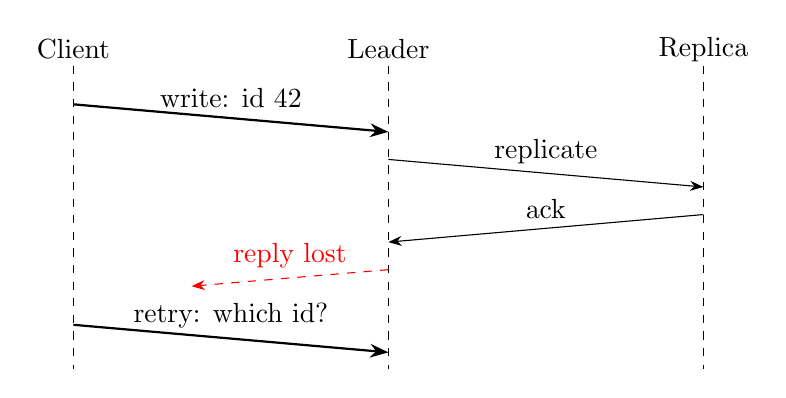
\begin{tikzpicture}[>=Stealth,x=1cm,y=.7cm]
\node at (0,0) {Client};\node at (4,0) {Leader};\node at (8,0) {Replica};
\draw[dashed] (0,-.3)--(0,-5.8) (4,-.3)--(4,-5.8) (8,-.3)--(8,-5.8);
\draw[->,thick] (0,-1)--node[above]{write: id 42}(4,-1.5);
\draw[->] (4,-2)--node[above]{replicate}(8,-2.5);
\draw[->] (8,-3)--node[above]{ack}(4,-3.5);
\draw[->,red,dashed] (4,-4)--node[above]{reply lost}(1.5,-4.3);
\draw[->,thick] (0,-5)--node[above]{retry: which id?}(4,-5.5);
\end{tikzpicture}
\end{frame}
\begin{frame}{Separate three failure hypotheses}
\begin{enumerate}[<+->]
\item The request never reached the service.
\item The service received it but did not commit it.
\item The service committed it but the response was lost.
\end{enumerate}
\begin{block}{Evidence gap}
A client timeout is compatible with all three. An application retry policy must handle that ambiguity.
\end{block}
\end{frame}
\section{Explain}
\begin{frame}{Replication and request identity solve different problems}
\begin{description}
\item[Replicated log] Establish an agreed order of state-machine commands.
\item[Request identity] Connect a retry to the same logical operation.
\item[Durable deduplication] Preserve the result needed to answer a repeated identity.
\end{description}
Consensus alone does not make an external email or payment endpoint idempotent.
\end{frame}
\begin{frame}{Majority intersection is a safety ingredient}
For $n$ replicas, take quorum size $q=\lfloor n/2\rfloor+1$.
\[
 |Q_1\cap Q_2|\geq |Q_1|+|Q_2|-n=2q-n>0.
\]
\pause
\begin{alertblock}{Necessary context}
Intersection alone is not a consensus protocol. Terms, voting rules, log checks and persistence determine what that shared replica may accept.
\end{alertblock}
\end{frame}
\begin{frame}[fragile]{Review a retry policy as application code}
\begin{lstlisting}[language=Python]
request_id = new_id()           # outside the retry loop
for attempt in range(3):
    try:
        return service.apply(request_id, command)
    except Timeout:
        backoff(attempt)
raise OutcomeUnknown(request_id)
\end{lstlisting}
\small Sketch only: the service must atomically bind the identity to the operation and its result. A bounded retry can still finish with an unknown outcome.
\end{frame}
\section{Respond}
\begin{frame}{The incident action list should be testable}
\begin{tabular}{p{.27\textwidth}p{.62\textwidth}}
\textbf{Inject} & Drop the reply after a successful commit.\\[1ex]
\textbf{Assert} & A repeated identity returns the stored result without repeating the effect.\\[1ex]
\textbf{Observe} & Log request identity, outcome and retry count across process restarts.
\end{tabular}
\end{frame}
\begin{frame}{Close the review with two different guarantees}
\begin{block}{Safety question}
What bad state must never be produced, including after restart and retry?
\end{block}
\begin{exampleblock}{Liveness question}
Under which communication and availability assumptions can progress resume?
\end{exampleblock}
\small Background: Ongaro and Ousterhout, \href{https://raft.github.io/raft.pdf}{\emph{In Search of an Understandable Consensus Algorithm} (2014)}.
The scenario and retry sketch are original and do not constitute a complete Raft implementation.
\end{frame}
\end{document}
